\documentclass[11pt,a4paper]{article}
\author{TalentSprint}
\date{}
\usepackage{verbatim}
\usepackage{fancyhdr}           % For header and footer
\usepackage{multicol}
\usepackage{colortbl}           % For coloured tables
\usepackage{setspace}           % For line height
\usepackage{seqsplit}           % Splits long words.
\usepackage{amsmath} 
\usepackage{graphicx}
\usepackage{array}
\usepackage{enumitem}
\usepackage{xcolor}
\usepackage[tikz]{bclogo}
\usepackage{textcomp}
\usepackage{listings}
\lstset{language=python,numbers=left,numberstyle=\tiny,numbersep=10pt,showstringspaces=false}

\headheight=14pt
%\footheight=14pt
\lhead{\nouppercase{}}
\rhead{\nouppercase{\leftmark}}

\newcommand*\lstinputpath[1]{\lstset{inputpath=#1}}
\lstinputpath{../Code/}
\graphicspath{{../Images/} {../ScreenShots/}}

\setcounter{tocdepth}{1}
\setlength\parindent{0pt}
\parskip=4pt
\newcommand{\Code}[1]{\textbf{\texttt{#1}}}

% Lengths and widths
\addtolength{\textwidth}{5cm}
\addtolength{\hoffset}{-1cm}
\setlength{\headsep}{-12pt} % Reduce space between header and content
\setlength{\headheight}{85pt} % If less, LaTeX automatically increases it
\renewcommand{\footrulewidth}{2pt} % Remove footer line
\renewcommand{\headrulewidth}{1pt} % Remove header line
\renewcommand{\seqinsert}{\ifmmode\allowbreak\else\-\fi} % Hyphens in seqsplit
% This two commands together give roughly
% the right line height in the tables
\renewcommand{\arraystretch}{1.3}
\onehalfspacing

% Commands
\newcommand{\SetRowColor}[1]{\noalign{\gdef\RowColorName{#1}}\rowcolor{\RowColorName}} % Shortcut for row colour
\newcommand{\mymulticolumn}[3]{\multicolumn{#1}{>{\columncolor{white}}#2}{#3}} % For coloured multi-cols
\newcolumntype{x}[1]{>{\raggedright}p{#1}} % New column types for ragged-right paragraph columns
\newcommand{\tn}{\tabularnewline} % Required as custom column type in use

% Font and Colours
\definecolor{HeadBackground}{HTML}{333333}
\definecolor{FootBackground}{HTML}{666666}
\definecolor{TextColor}{HTML}{333333}
\definecolor{DarkBackground}{HTML}{6B8E23} %{FD1AA8}
\definecolor{LightBackground}{HTML}{E8FED8} %D3FDC8
\definecolor{tit}{HTML}{FF6600}
\renewcommand{\familydefault}{\sfdefault}
\color{TextColor}
 \headsep = 25pt
% Header and Footer
\pagestyle{fancy}
\usepackage[headheight=110pt]{geometry}
\fancyhf{}% Clear header/footer

\fancyhead[r]{
\includegraphics[width = 4cm, height = 2cm]{TS-Logo.png}\hspace{0cm}}

%=================================TITLE=====================================
\fancyhead[l]{\Large{\bf{\textcolor{tit}{\textrm{Looping Statements}}}}}
%===========================================================================

\renewcommand{\headrulewidth}{0.4pt}% Default \headrulewidth is 0.4pt
\renewcommand{\footrulewidth}{0.4pt}% Default \footrulewidth is 0pt

\rfoot{Page \thepage}
\lfoot{COPYRIGHT \textcopyright TALENTSPRINT, 2015. ALL RIGHTS RESERVED.}




\begin{document}


%\chapter{Looping Statements}
To print the numbers from 0 to 9, using what we have learnt so far, we can write the program like this:

\begin{lstlisting}
int main() {
    int i = 0;
    printf("%d\n", i);
    i++;
    printf("%d\n", i);
    i++;
    printf("%d\n", i);
    i++;
    printf("%d\n", i);
    i++;
    printf("%d\n", i);
    i++;
    printf("%d\n", i);
    i++;
    printf("%d\n", i);
    i++;
    printf("%d\n", i);
    i++;
    printf("%d\n", i);
    i++;
    printf("%d\n", i);
}
\end{lstlisting}

\subsection*{Need for loops} Of course no one will write code this way; nor should they. Still let us look at the problems that arise due to this sort of code:
\begin{itemize}
\item Increased code size
\item which leads to poor readability
\item makes changes difficult.
\end{itemize}
Of course we can imagine more issues of serious and not so serious impact, but the point is that we need a way to repeatedly execute the same code, rather than write the same code multiple times.

In other words, we need mechanism(s) to execute  a block of code several number of times. A loop is precisely such a mechanism.

A loop uses a condition to control the repetition. The repetition is done as long as the condition is \texttt{true}.

We can describe the general form of a loop as: 
\begin{itemize}
\item Declare and initialize a variable.
\item Check condition to start the loop
\item Executing statements inside loop.
\item Modify the value of the variable.
\end{itemize}

\section*{Types of Looping Statements}
C provides three looping constructs:
\begin{description}
\item[while] The most general construct. Should be used when you want to repeatedly execute a set of statements based on the condition. 
\item[for] The counting loop. In C there is no effective difference between \lstinline!for! and \lstinline!while!.  A \lstinline!for! loop can be rewritten as a \lstinline!while! and vice versa. But it is strongly recommended that you use the for only in situatons you want to loop a (known) number of times.
\item[do \ldots while] The least used construct. Is useful only in very special situation where you want to run the body of the loop at least once.
\end{description}

\section*{While Loop}
A \lstinline!while! loop repeatedly executes target statement(s) \emph{as long as} a given condition is true.

\subsection*{Syntax}
\begin{lstlisting}[numbers=none]
  while (boolean_expression) {
    statement(s);
  }
\end{lstlisting}
\begin{figure}[ht]
\begin{center}
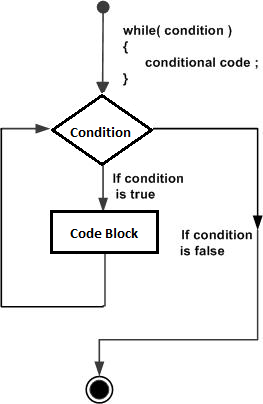
\includegraphics[scale=0.7]{while_loop.png}
\caption{Flow Chart: while}
\label{Flowchart:while}
\end{center}
\end{figure}

\subsection*{Explanation}
\begin{itemize}
\item Here, \texttt{statement(s)} may be one statement or a block.
\item The boolean\_expression is checked; if true the statement(s) are executed. 
\item Then the condition is checked again; the cycle repeats till the condition becomes false.
\item When the condition becomes false,  program control passes to the line immediately following the loop.
\item In \texttt{while} loop the statement(s) may not execute even once, if the condition is \texttt{false} the first time.
\end{itemize}

\begin{bclogo}[couleur=blue!5, arrondi=0.3, logo=\bcattention]{Warning}
The condition must change due to the effect of the loop body. Otherwise the loop will \textsc{never} stop. In other words, there must be at least one statement in the loop body that affects the condition. 
\end{bclogo}

\subsubsection*{Example}

A program to print numbers from 1 to 10.
\lstinputlisting{Program-07-1.c}

\begin{figure}[ht]
\begin{center}
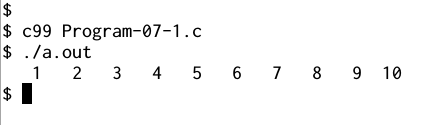
\includegraphics[scale=0.6]{Output-07-1.png}
\caption{Printing 1-10 in a while loop}
\label{output-07-1}
\end{center}
\end{figure}

\subsubsection*{Example}
 A program to print all even numbers within a given range.
\lstinputlisting{Program-07-2.c}

\begin{figure}[ht]
\begin{center}
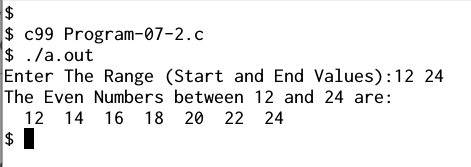
\includegraphics[scale=0.6]{Output-07-2.png}
\caption{Printing a range of even numbers}
\label{output-07-2}

\end{center}
\end{figure}

\section*{For Statement}
A \lstinline!for! is a looping control structure that allows you to efficiently write a loop that needs to execute a specified number of times.

\subsection*{Syntax}
\begin{lstlisting}[numbers=none]
for (initialization; condition; increment) {
    statement(s);
}
\end{lstlisting}
\begin{figure}[ht]

\begin{center}
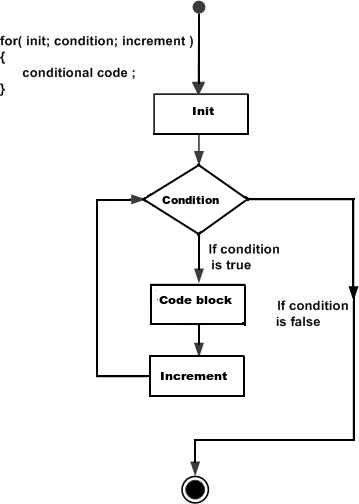
\includegraphics[scale=0.5]{for_loop.png}
\caption{Flowchart: for}
\label{Flowchart:for}
\end{center}
\end{figure}

\subsection*{Explanation} 
Here is the flow of control in a \lstinline!for! loop
\begin{enumerate}
\item The \textbf{initialization} step is executed first, and only once. 
  \begin{itemize}
  \item While this can be any executable statement, idiomatically it must be used to declare and initialize the loop control variable(s). 
  \item It can even be an empty statement -- but there must be a semicolon as the first non-space character inside the parentheses.
  \end{itemize}
\item Next, the \textbf{condition} is evaluated. If it is \texttt{true}, the body of the loop is executed. If it is \texttt{false}, control directly passes to the next statement \emph{after} the \lstinline!for! loop.
\begin{itemize}
  \item In other words, a \lstinline!for! loop may not execute the body of statements even once.
\end{itemize}
\item After the body of the \lstinline!for! loop executes, control is transferred to the \textbf{increment} statement. 
\begin{itemize}
  \item Once again, like the initialization statement, it can be any executable statement or empty. Idiomatically, this  statement must modify loop control variable(s), thus controlling how many times the loop is executed.
    \item We have called it increment; but it can be a decrement or any other statement that modifies the value of the index variable.
\end{itemize}
\item The condition is now evaluated again. If it is true, the loop executes and the process repeats itself (body of loop, then increment step, and then  condition check). When the condition becomes false, the \lstinline!for! loop terminates.
\end{enumerate}

\subsection*{Example}
Program to print the multiplication table of a given number.
\lstinputlisting{Program-07-3.c}

\begin{figure}[ht]
\begin{center}
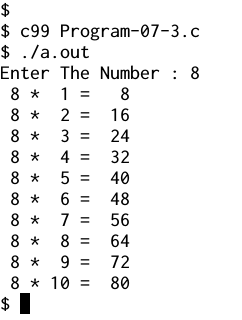
\includegraphics[scale=0.6]{Output-07-3.png}
\caption{Multiplication Table}
\label{output-07-3}
\end{center}
\end{figure}

\subsection*{Example} 
\lstinputlisting{Program-07-4.c}

\begin{figure}[ht]
\begin{center}
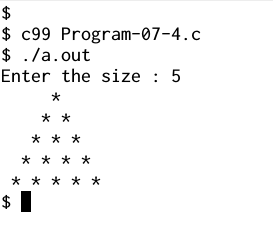
\includegraphics[scale=0.6]{Output-07-4.png}
\caption{Building a pattern}
\label{output-07-4}
\end{center}
\end{figure}

\section*{Break and Continue}
There are two statements available in C, \lstinline{break} and \lstinline{continue} to change the control flow of a loop. Loops perform a set of operations repeatedly until certain condition is met but, it is sometimes desirable to skip some statements inside the loop or terminate the loop. In such cases, \lstinline!break! and \lstinline!continue! statements are used.

\subsection*{Break Statement}
It is used to terminate the loop immediately after a certain condition encountered. This condition is different from the loop's condition. Thus the \lstinline!break! statement is used with conditional \lstinline!if! statement.

\subsection*{Example}
Program to print the numbers between the given range, terminating the loop if it encounters a number that is a factor of 10.

\lstinputlisting{Program-07-5.c}

A natural question arises: `Why use a separate condition? Why not combine it with loop condition?' We want to print the multiple of 10 \emph{and then exit}. This means we need to check after printing. 

More realistically, the condition for deciding on the \lstinline!break! would depend on the computations made inside the loop and hence the checking has to be done after the relevant lines of code.

\begin{figure}[ht]
\begin{center}
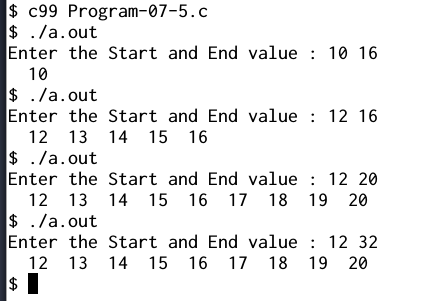
\includegraphics[scale=0.6]{Output-07-5.png}
\caption{Stop print at 10n}
\label{output-07-5}
\end{center}
\end{figure}

\subsection*{Continue Statement} 
The \lstinline!continue! statement is used to skip over the rest of the loop iteration and directly jump to the loop control. Will start the next iteration immediately.

\subsubsection*{Example}

Program to print the sum of all odd numbers between the given range.

\lstinputlisting{Program-07-6.c}

\begin{figure}[ht]
\begin{center}
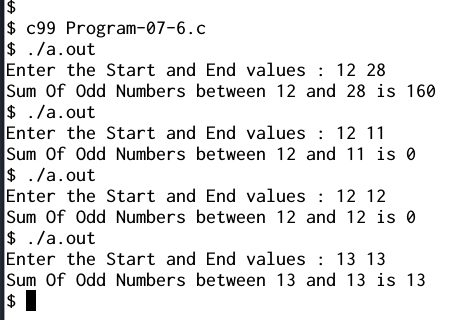
\includegraphics[scale=0.6]{Output-07-6.png}
\caption{Odd numbers: using Continue}
\label{output-07-6}
\end{center}
\end{figure}

\section*{do \ldots while Loop}
The \lstinline!for! and \lstinline!while! loops  test the loop condition at the top of the loop.
The \lstinline!do! \ldots \lstinline!while! loop in C programming language checks its condition at the bottom of the loop.

A \lstinline!do! \ldots \lstinline!while! loop is similar to a \lstinline!while! loop, except that the body of the \lstinline!do! \ldots \lstinline!while! loop is guaranteed to execute at least once.

\subsection*{Syntax}
\begin{verbatim}
    do {
        statement(s);
    } while (boolean_expression);
\end{verbatim}

\begin{figure}[ht]
\label{FlowChart do while}
\begin{center}
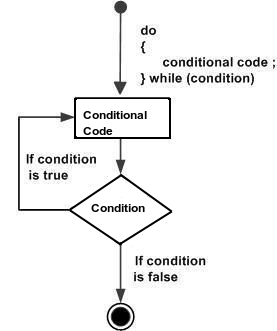
\includegraphics[scale=0.6]{dowhilefc.jpg}
\caption{FlowChart: do ... while}
\end{center}
\end{figure}

\subsection*{Example}
The following example illustrates how to use the \lstinline!do ... while! loop.
\lstinputlisting{Program-07-7.c}
\begin{figure}[ht]
\caption{do while output}
\label{output-07-7}
\begin{center}
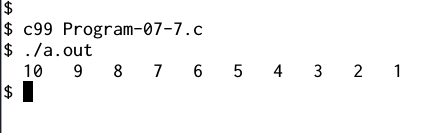
\includegraphics[scale=0.6]{Output-07-7.png}
\end{center}
\end{figure}

\section*{Nested Loops}
We can use one loop (of any kind) inside another loop (of any kind). This is known as \emph{nested} loop. The syntax for some possible nested loops is given below: 

\begin{lstlisting}[numbers=none]
  for (init; condition1; increment) {
    statement(s);
    while (condition2) {
      statement(s);
    }
    statement(s);
  }
\end{lstlisting}


\begin{lstlisting}[numbers=none]
  do {
    statement(s);
    for (init; condition1; increment) {
      statement(s);
    } 
    statement(s);
  } while(condition2);
\end{lstlisting}

\end{document}